\section*{QUESTION \quesNo.}

\subsection*{Explanation/Theory}

\[\] \vspace{-40px}

(a) Write the differential equation of the system in terms of $\omega_a$ and $\mathrm{Q}$. \\


To write the differential equation of the system, we start with the standard second-order linear differential equation for a damped harmonic oscillator:

\[
    M\ddot{x} + D\dot{x} + Kx = 0
\]

The above equations only states that sum of all forces in all the direction is zero.

To write the above equation in terms of $\omega_a$ and $\mathrm{Q}$, we use the given facts:

\[
    \omega_a = \sqrt{\frac{K}{M}} \Rightarrow K = M\omega_a^2
\]
\[
    \mathrm{Q} = \frac{\sqrt{KM}}{D} \Rightarrow D = \frac{\sqrt{KM}}{\mathrm{Q}} = \frac{M\omega_a}{\mathrm{Q}}
\]

Substituting the above expressions in the differential equation, we get:

\[
    \ddot{x} + \frac{\omega_a}{\mathrm{Q}}\dot{x} + \omega_a^2x = 0
\]

\[\] \vspace{-40px}

(b) Find the frequency response of the system. \\

For a given input $x(t)$ let the response of the system be $y(t)$. Thus above differential equation can be written as:

\[
    \ddot{y} + \frac{\omega_a}{\mathrm{Q}}\dot{y} + \omega_a^2y = x(t)
\]

Now let CTFT of $x(t)$ and $y(t)$ be $X(j\omega)$ and $Y(j\omega)$ respectively. Then the above equation can be written in frequency domain as:

\[
    (j\omega)^2 Y(j\omega) + \frac{\omega_a}{\mathrm{Q}}(j\omega)Y(j\omega) + \omega_a^2Y(j\omega) = X(j\omega) \\
\]
\[
    \left[ (j\omega)^2 + \frac{\omega_a}{\mathrm{Q}}(j\omega) + \omega_a^2 \right] \cdot Y(j\omega) = X(j\omega)
\]

Now to calculate the frequency response $H(j\omega)$:

\[
    H(j\omega) = \frac{Y(j\omega)}{X(j\omega)} = \frac{1}{(j\omega)^2 + \frac{\omega_a}{\mathrm{Q}}(j\omega) + \omega_a^2}
\]

This required frequency response is:

\[
    H(j\omega) = \frac{1}{(j\omega)^2 + \frac{\omega_a}{\mathrm{Q}}(j\omega) + \omega_a^2}
\]


\subsection*{MATLAB Code}

\lstinputlisting[
    style=Matlab-Pyglike
]{./matlab/22016_\quesNo.m}


\subsection*{Output}

\begin{figure}[H]
    \centering
    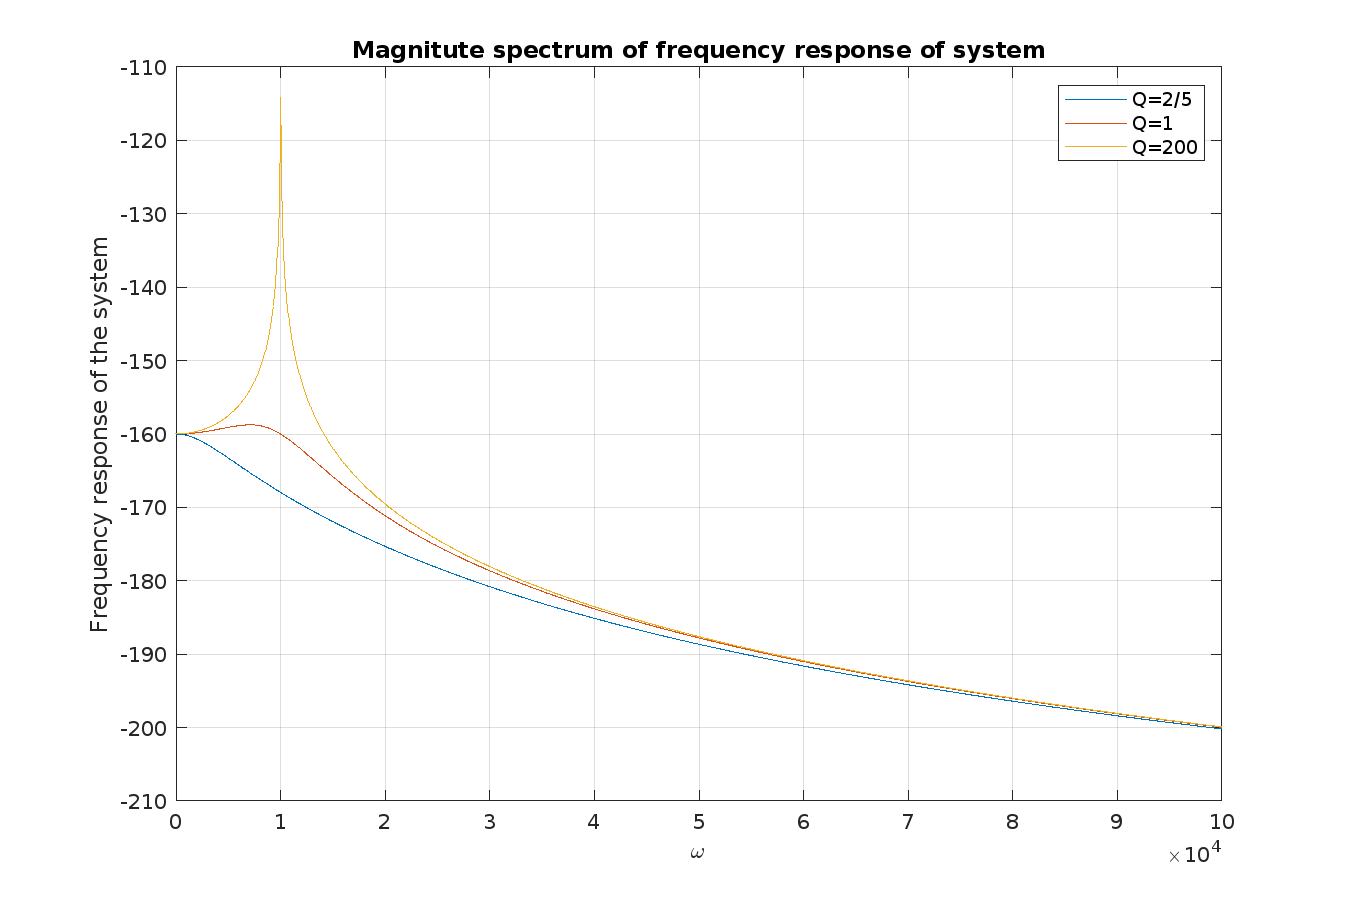
\includegraphics[width = \textwidth]{./imgs/3_mems_freq_resp.png}
\end{figure}

\pagebreak
\subsection*{Inference}

The frequency response of the system was plotted and we can infer the following:

\begin{enumerate}
    \item The frequency response for $\mathrm{Q} = 2/5$ decreases monotonically as increase in frequency $\omega$.
    \item The frequency response for $\mathrm{Q} = 1$ remains more or less constant for $\omega$ in range $[0, 1e4]$. After that it decreases.
    \item The frequency response for $\mathrm{Q} = 200$ has a sudden spike at $1e4$, before that it increases and after that it decreases.
\end{enumerate}

The system is an Damped Harmonic Oscillator and the frequency response is as expected.